\appendix{Представление графического материала}

Графический материал, выполненный на отдельных листах,
изображен на рисунках А.1--А.\arabic{числоПлакатов}.
\setcounter{числоПлакатов}{0}
\setcounter{figure}{0}

\renewcommand{\thefigure}{А.\arabic{figure}} % шаблон номера для плакатов

\begin{landscape}

\begin{плакат}
    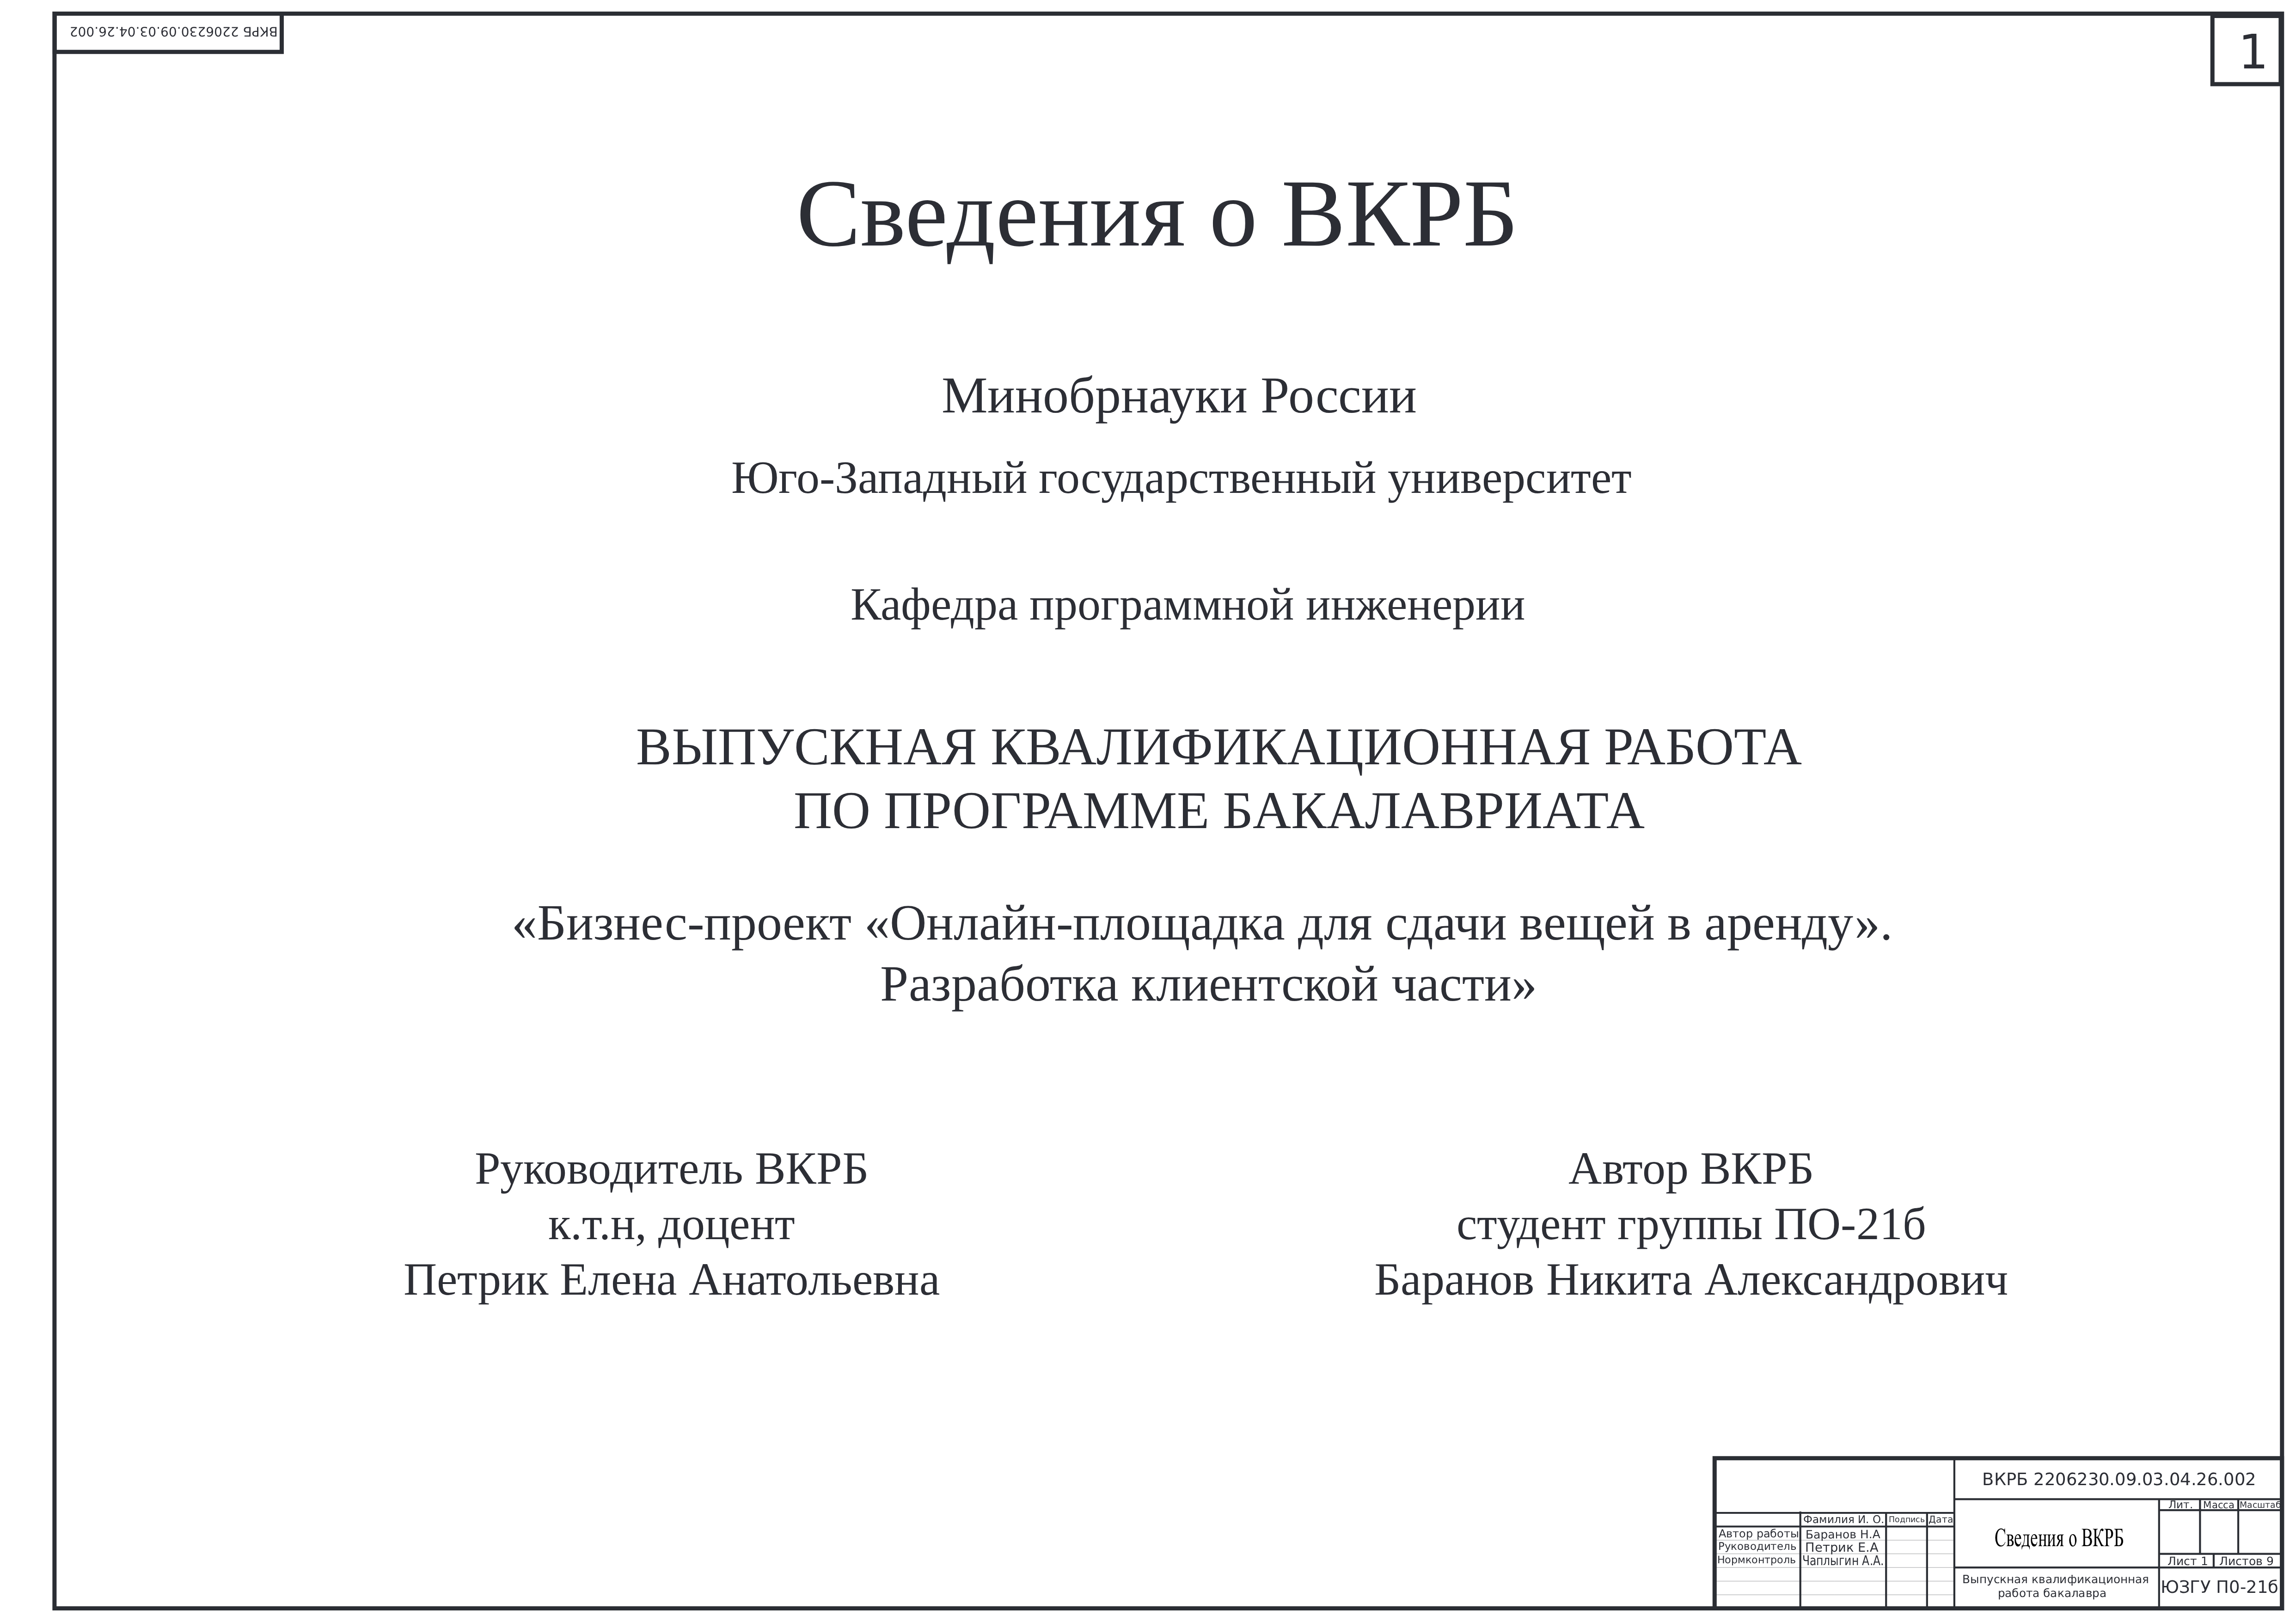
\includegraphics[width=0.82\linewidth]{Titulnik.png}
    \заголовок{Сведения о ВКРБ}
    \label{pl1:image}      
\end{плакат}

\begin{плакат}
    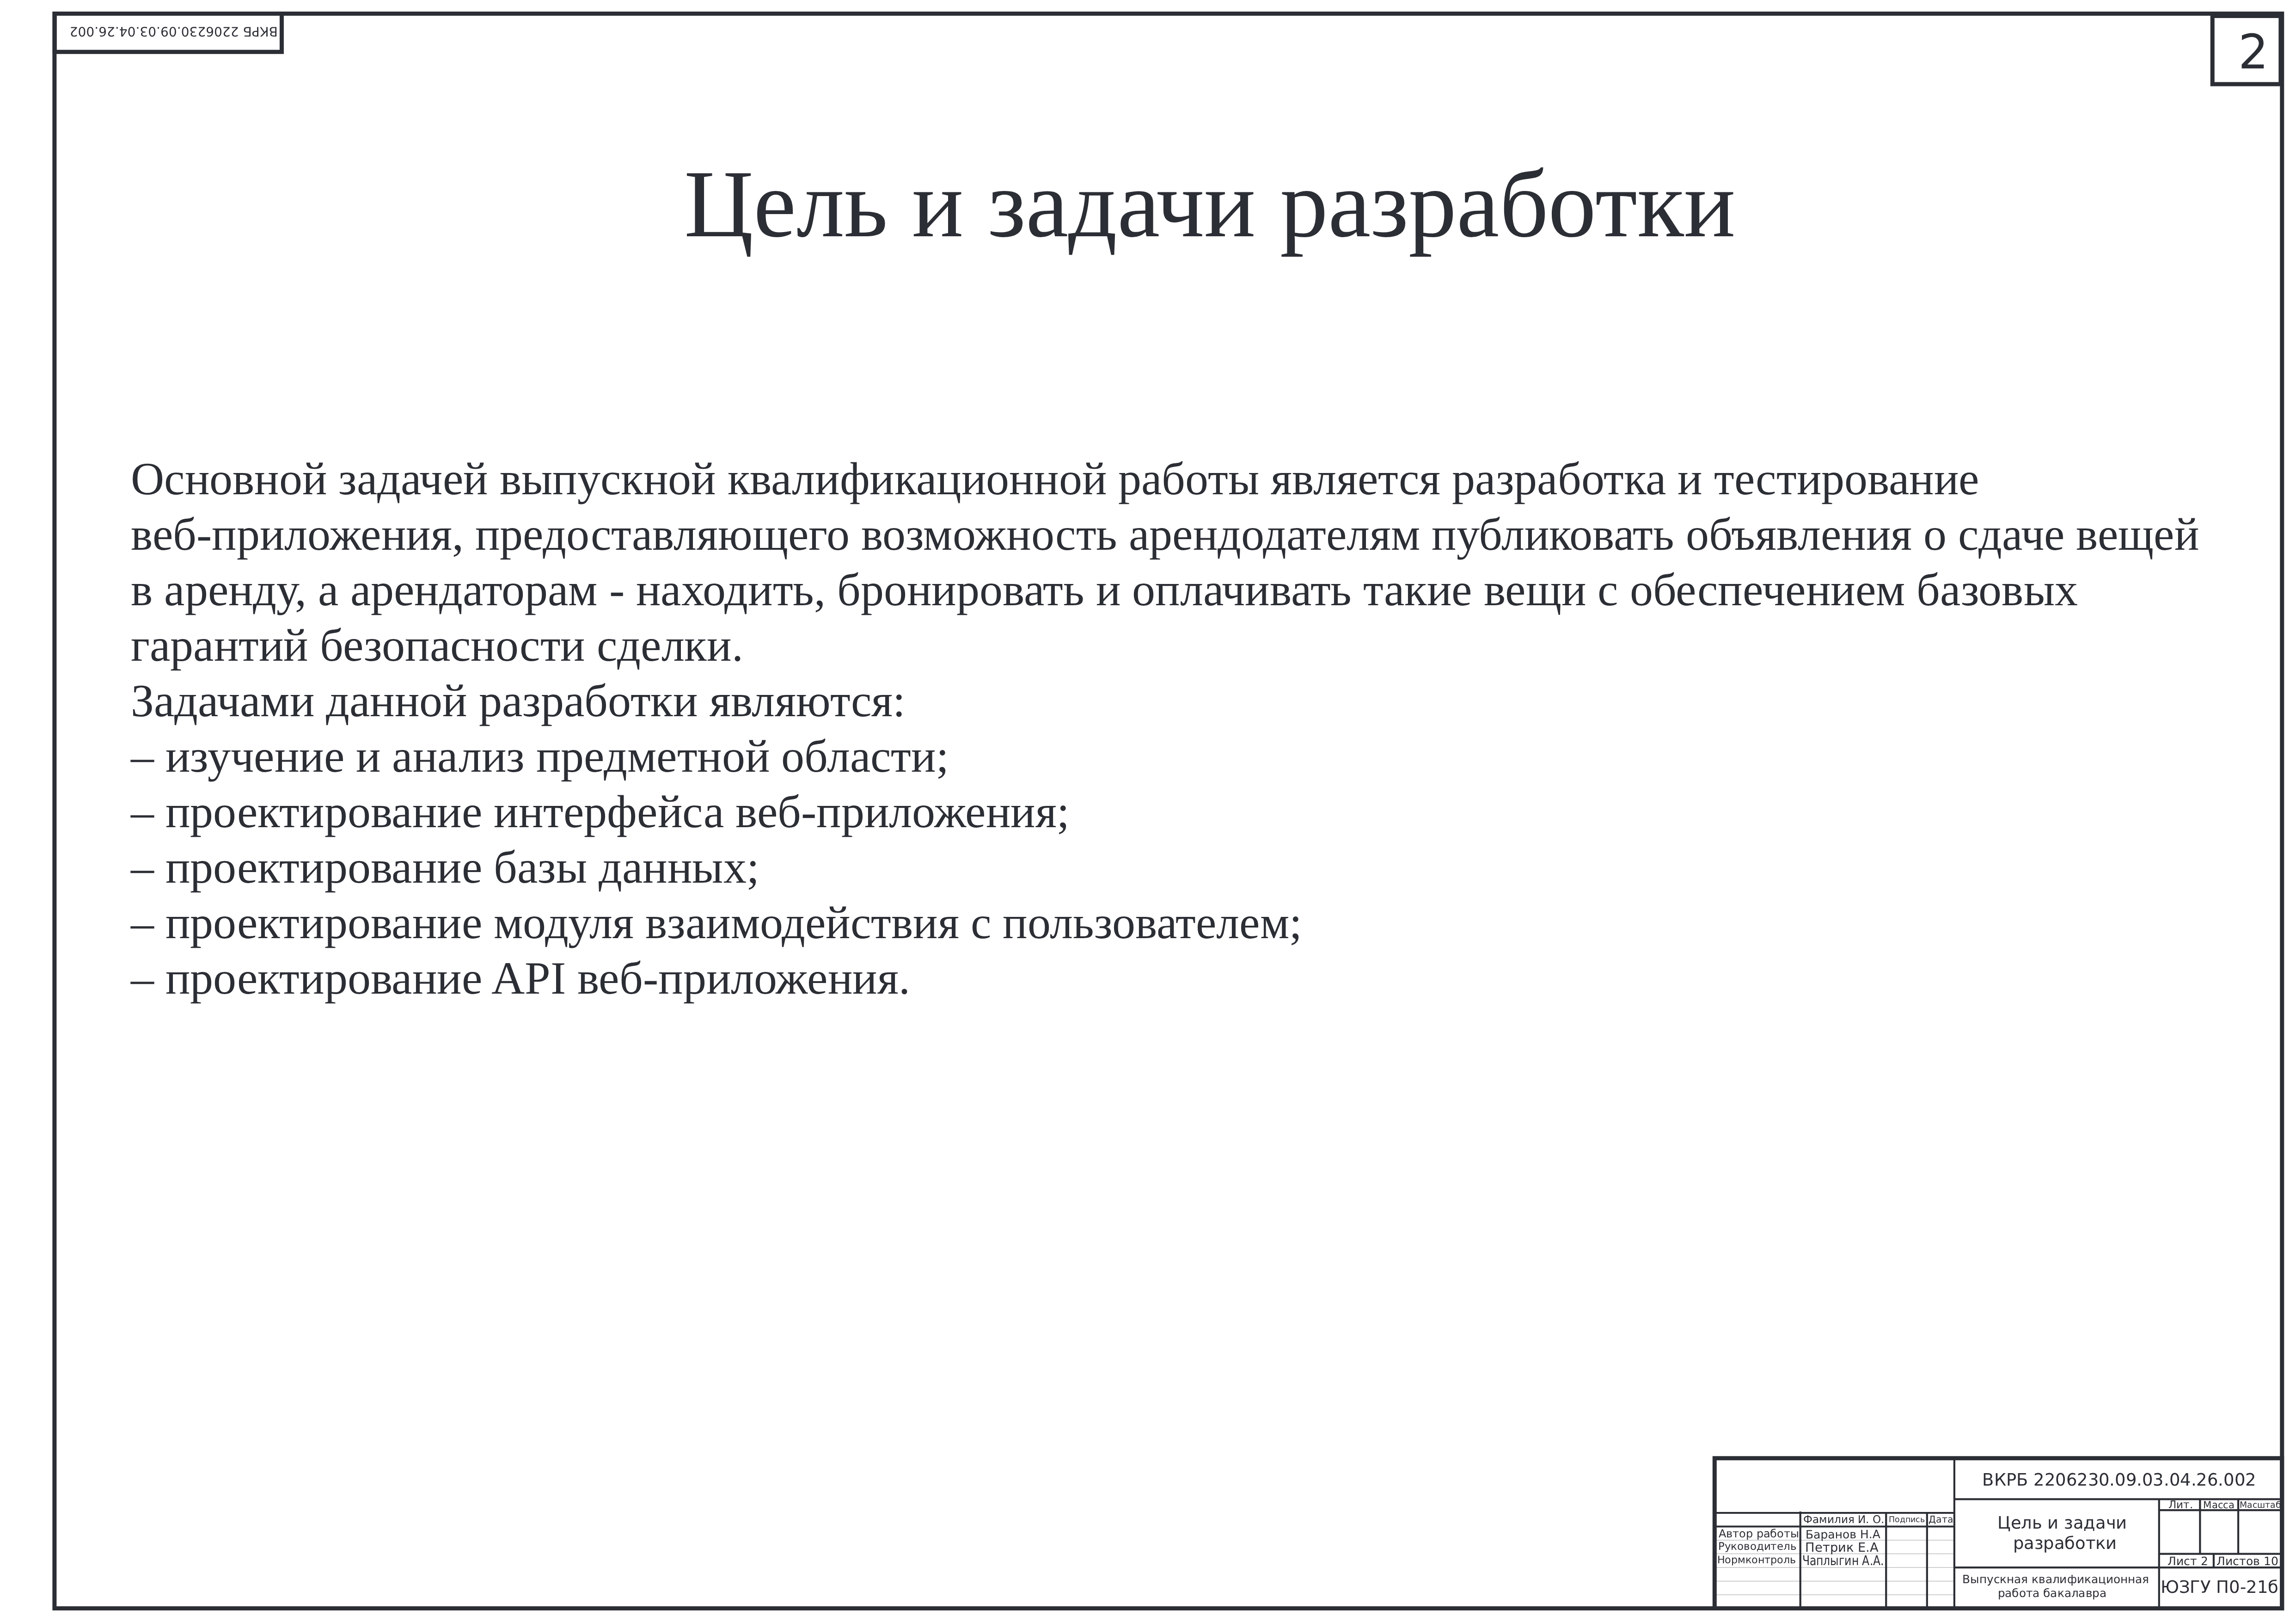
\includegraphics[width=0.82\linewidth]{Targets.png}
    \заголовок{Цель и задачи разработки}
    \label{pl2:image}      
\end{плакат}

\begin{плакат}
    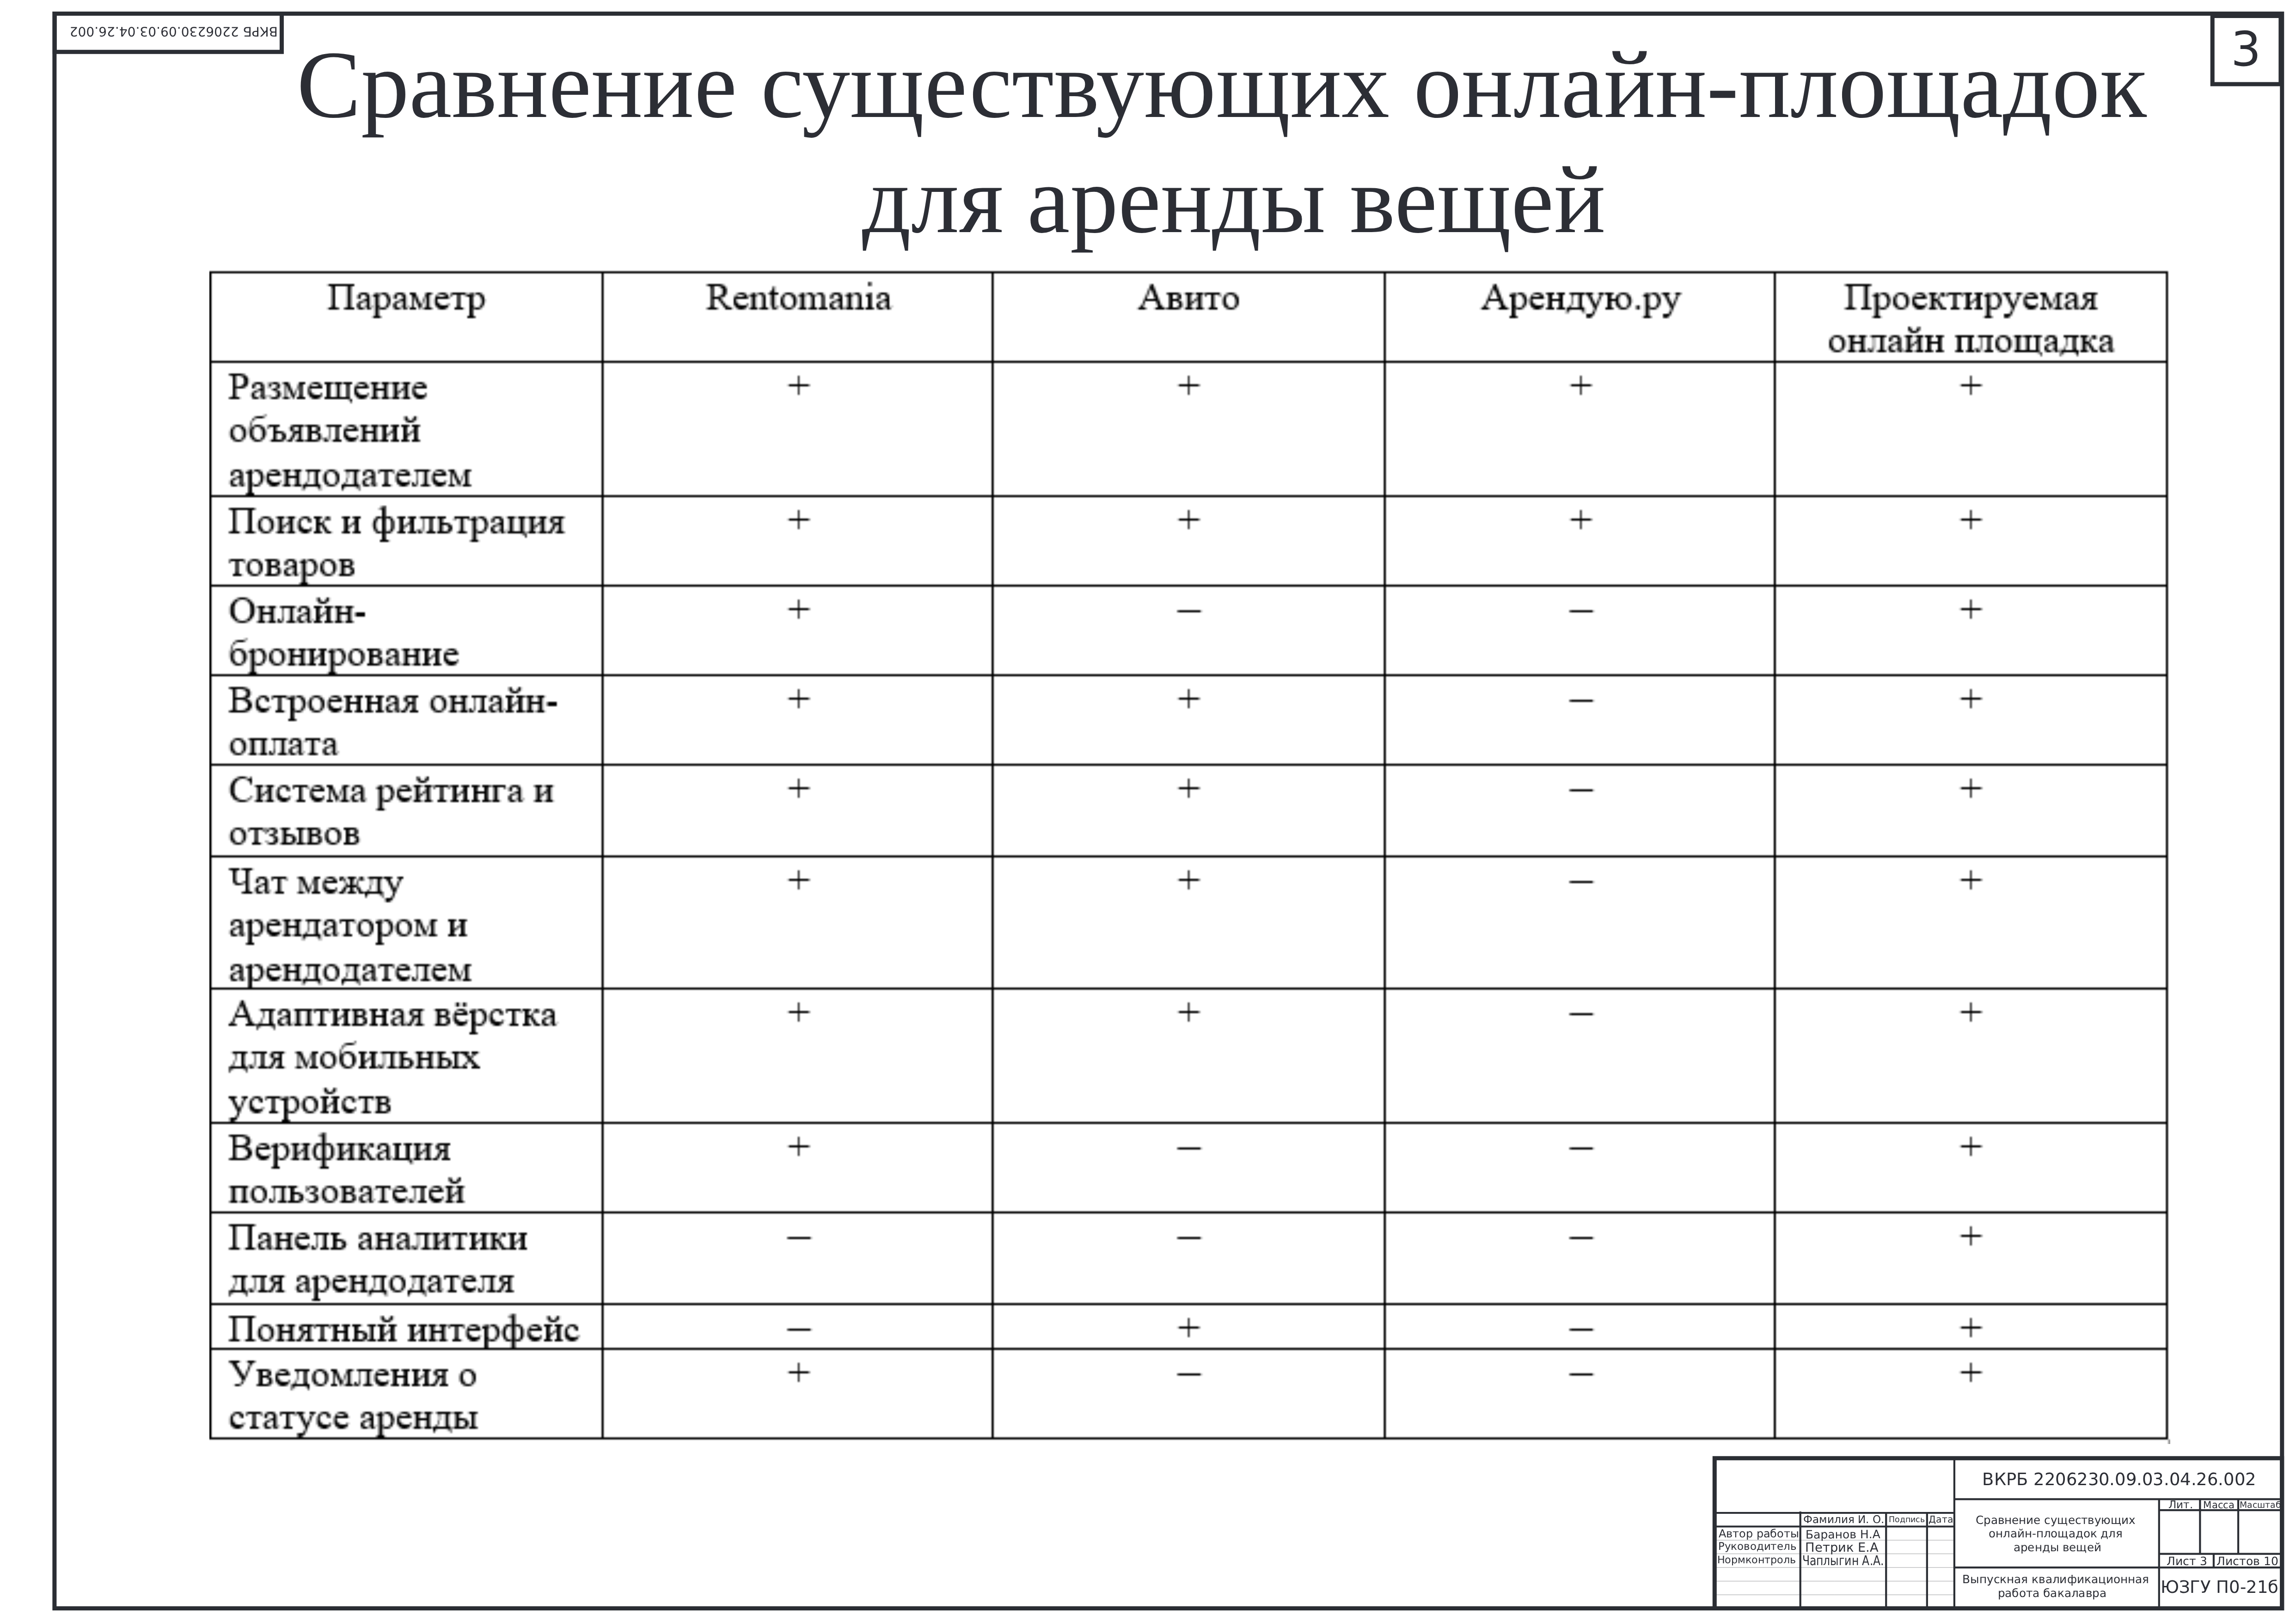
\includegraphics[width=0.82\linewidth]{Concurent.png}
    \заголовок{Сравнение конкурентов}
    \label{pl3:image}      
\end{плакат}

\begin{плакат}
    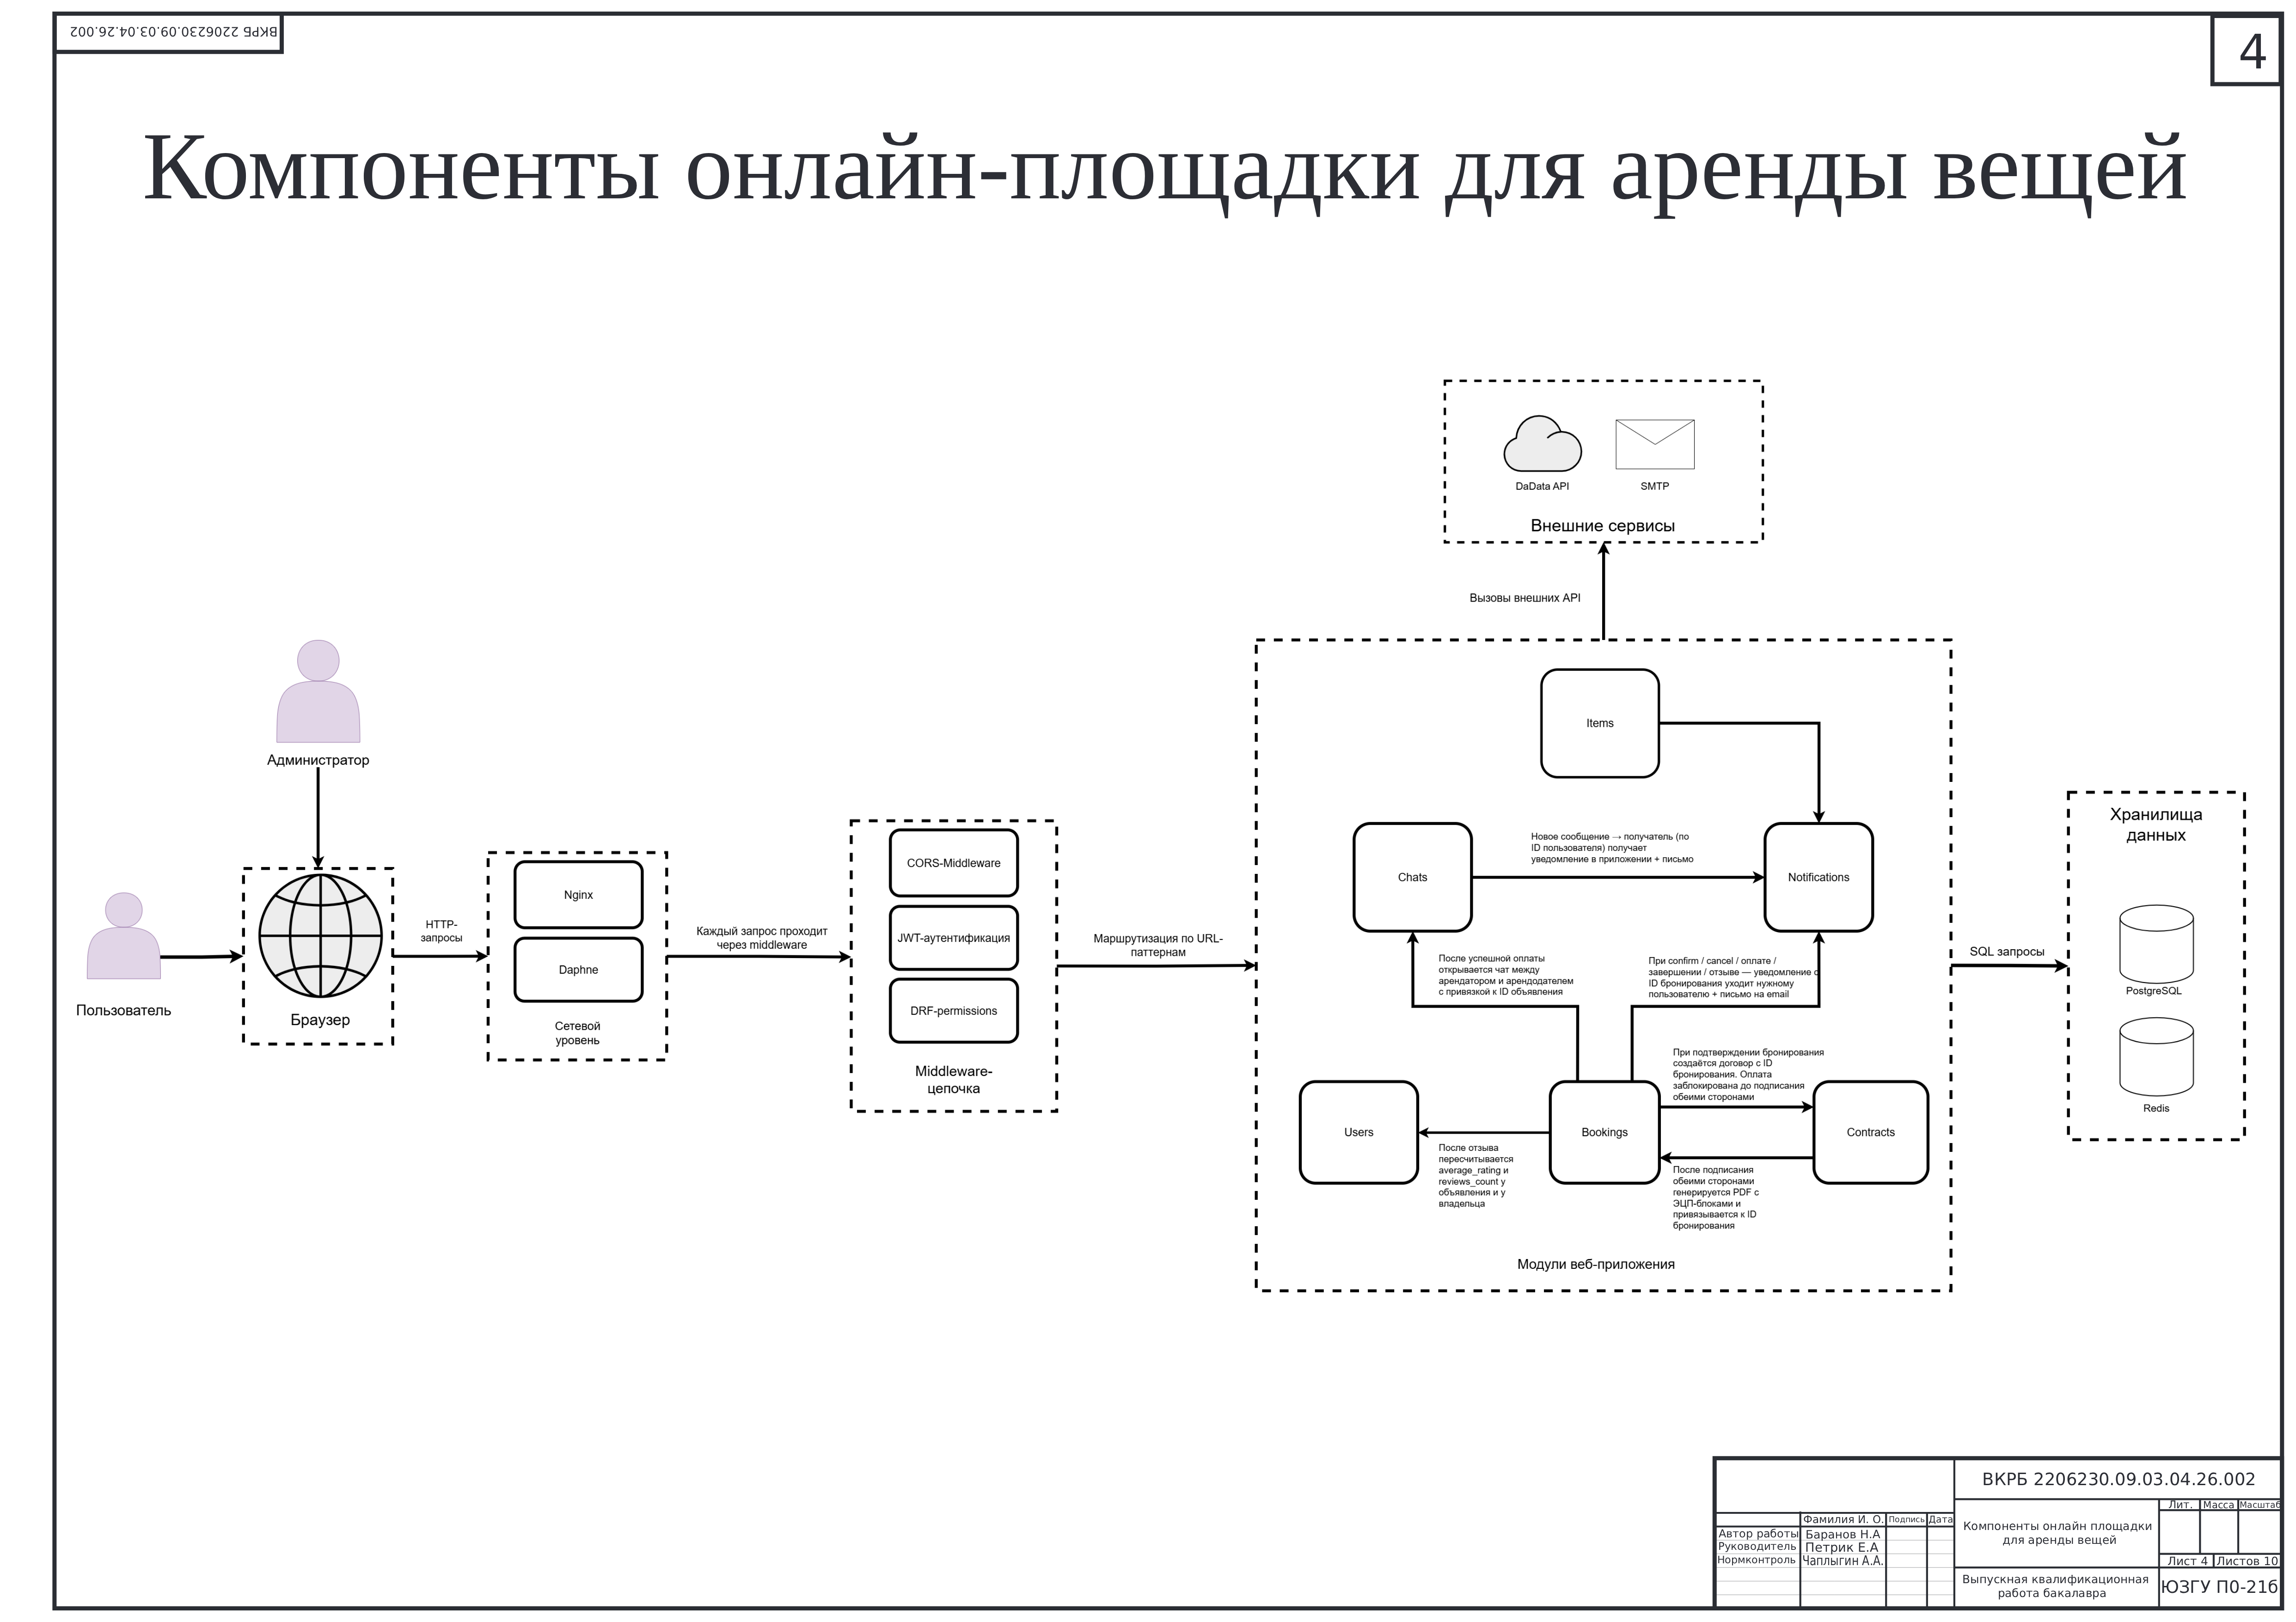
\includegraphics[width=0.82\linewidth]{Components.png}
    \заголовок{Компоненты онлайн-площадки для аренды вещей}
    \label{pl4:image}      
\end{плакат}

\begin{плакат}
    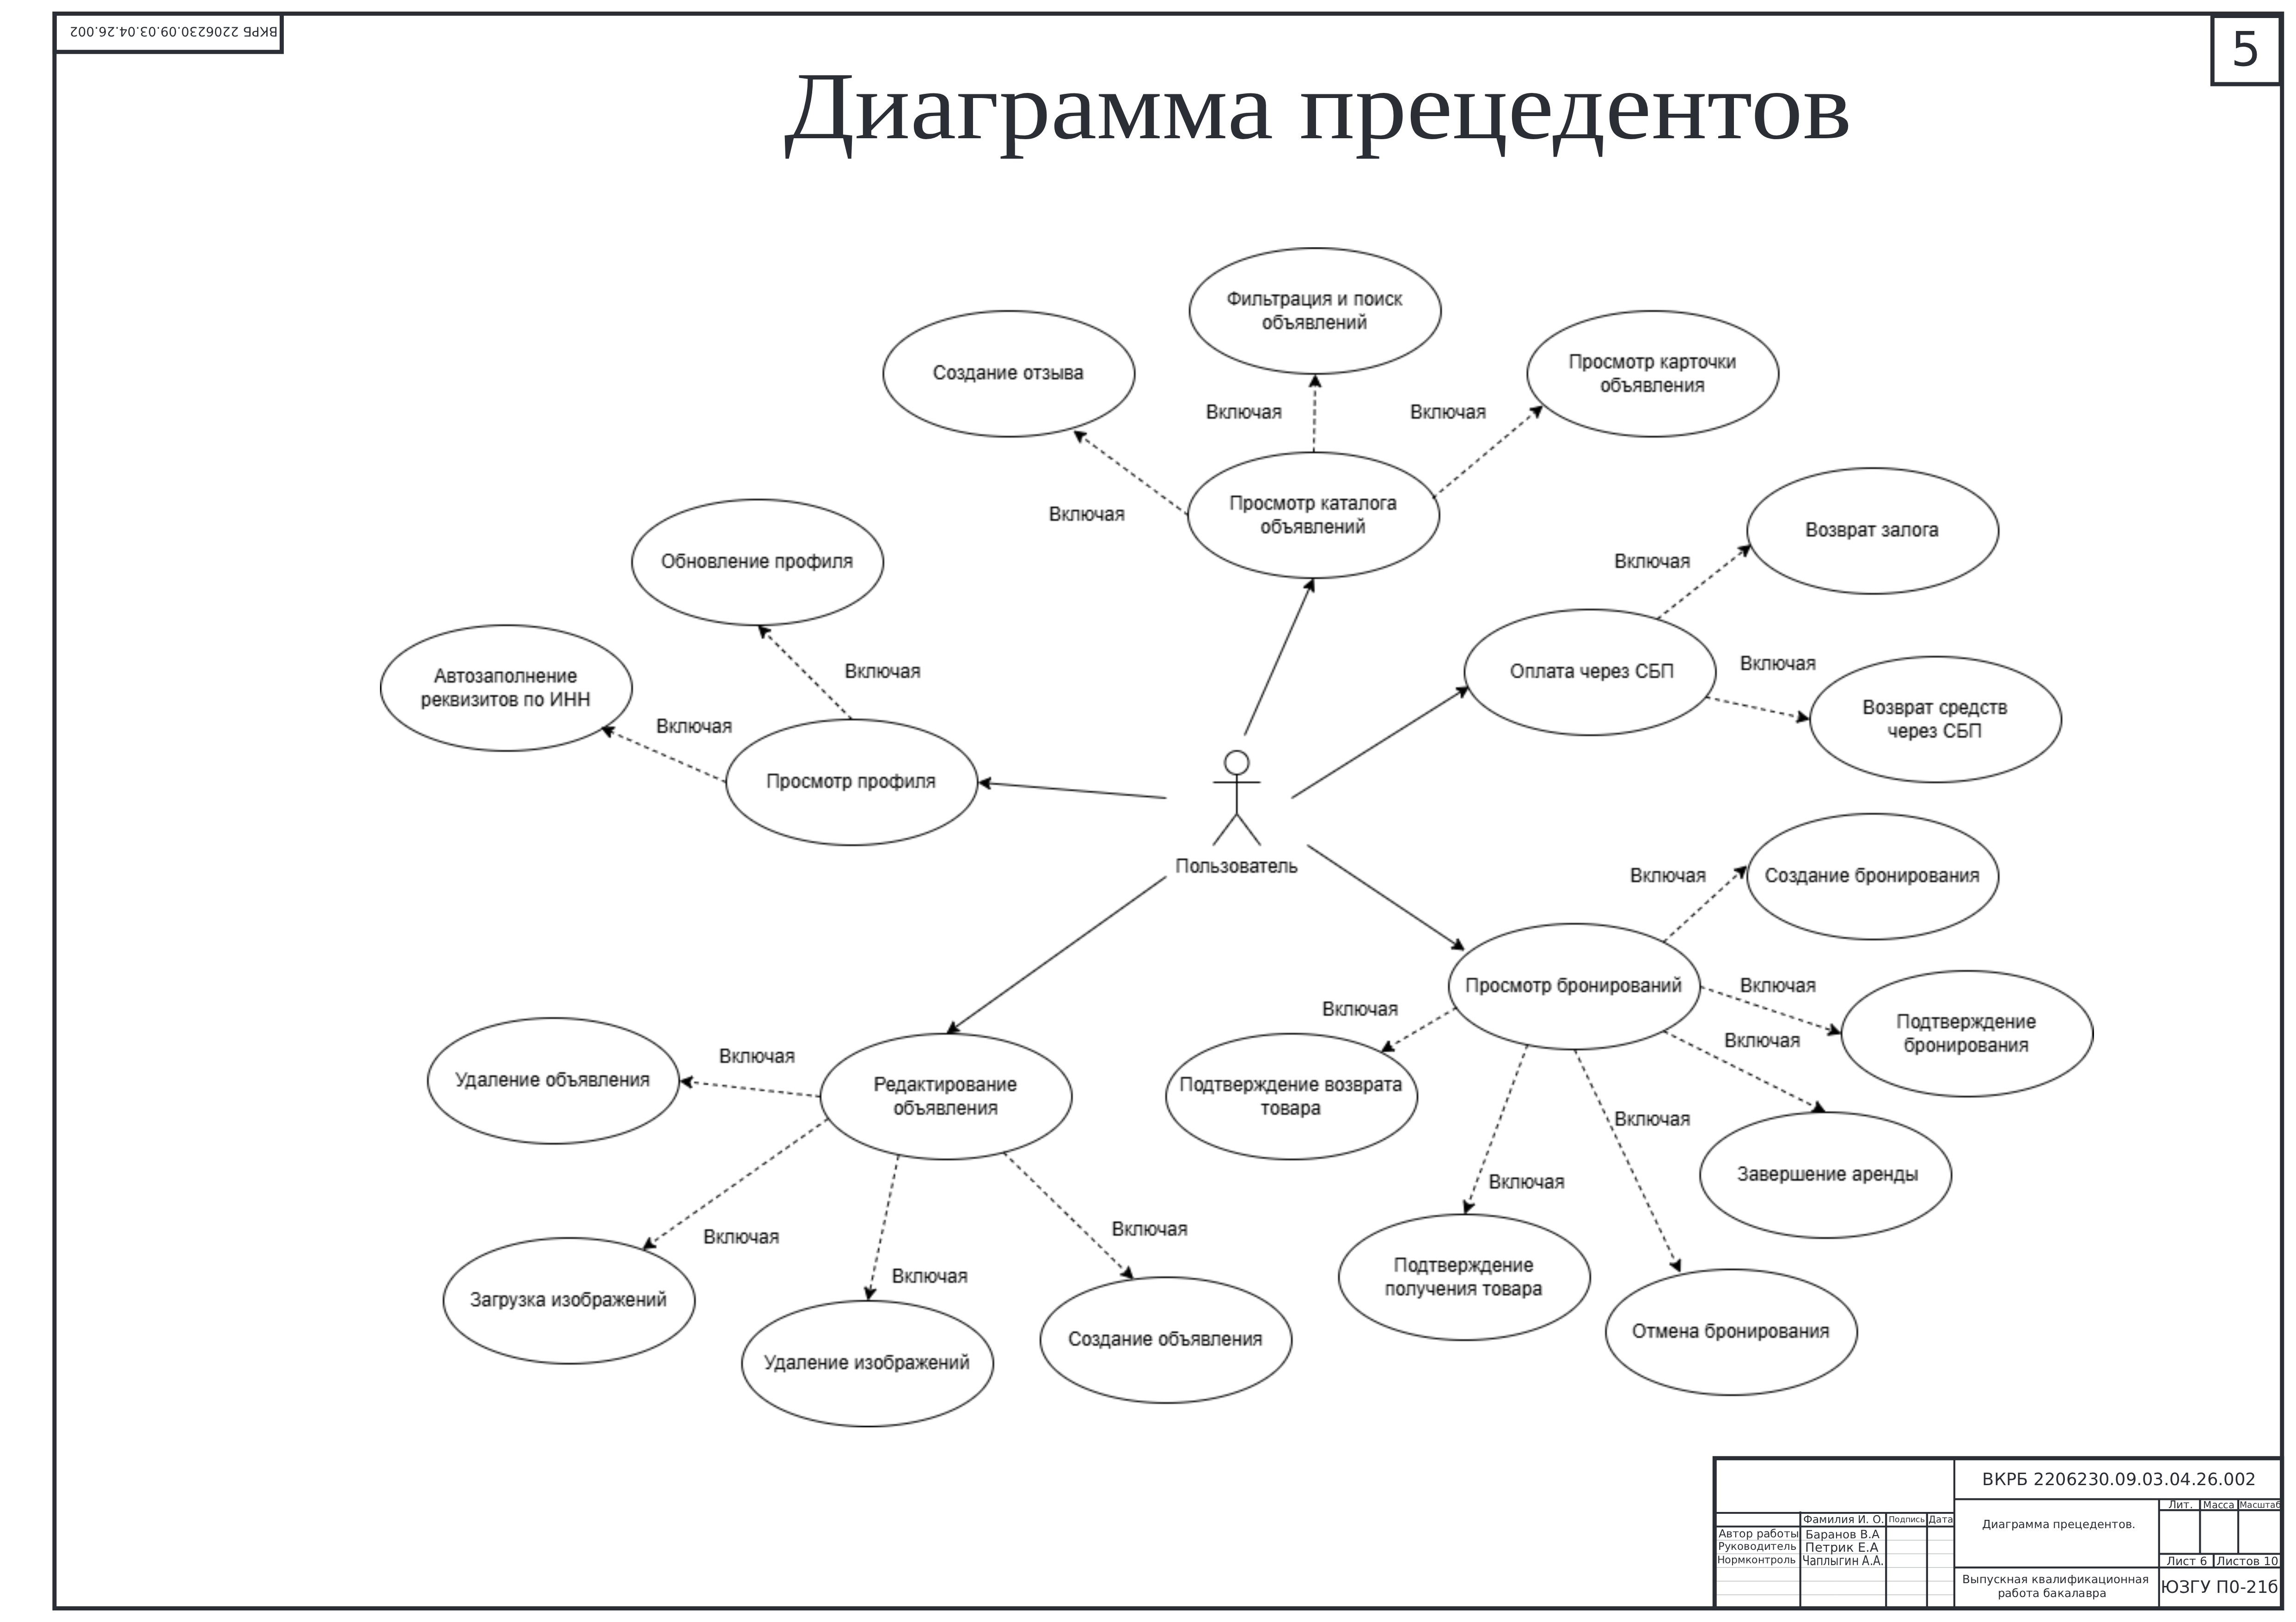
\includegraphics[width=0.82\linewidth]{precedents.png}
    \заголовок{Диаграмма прецедентов}
    \label{pl5:image}      
\end{плакат}

\begin{плакат}
    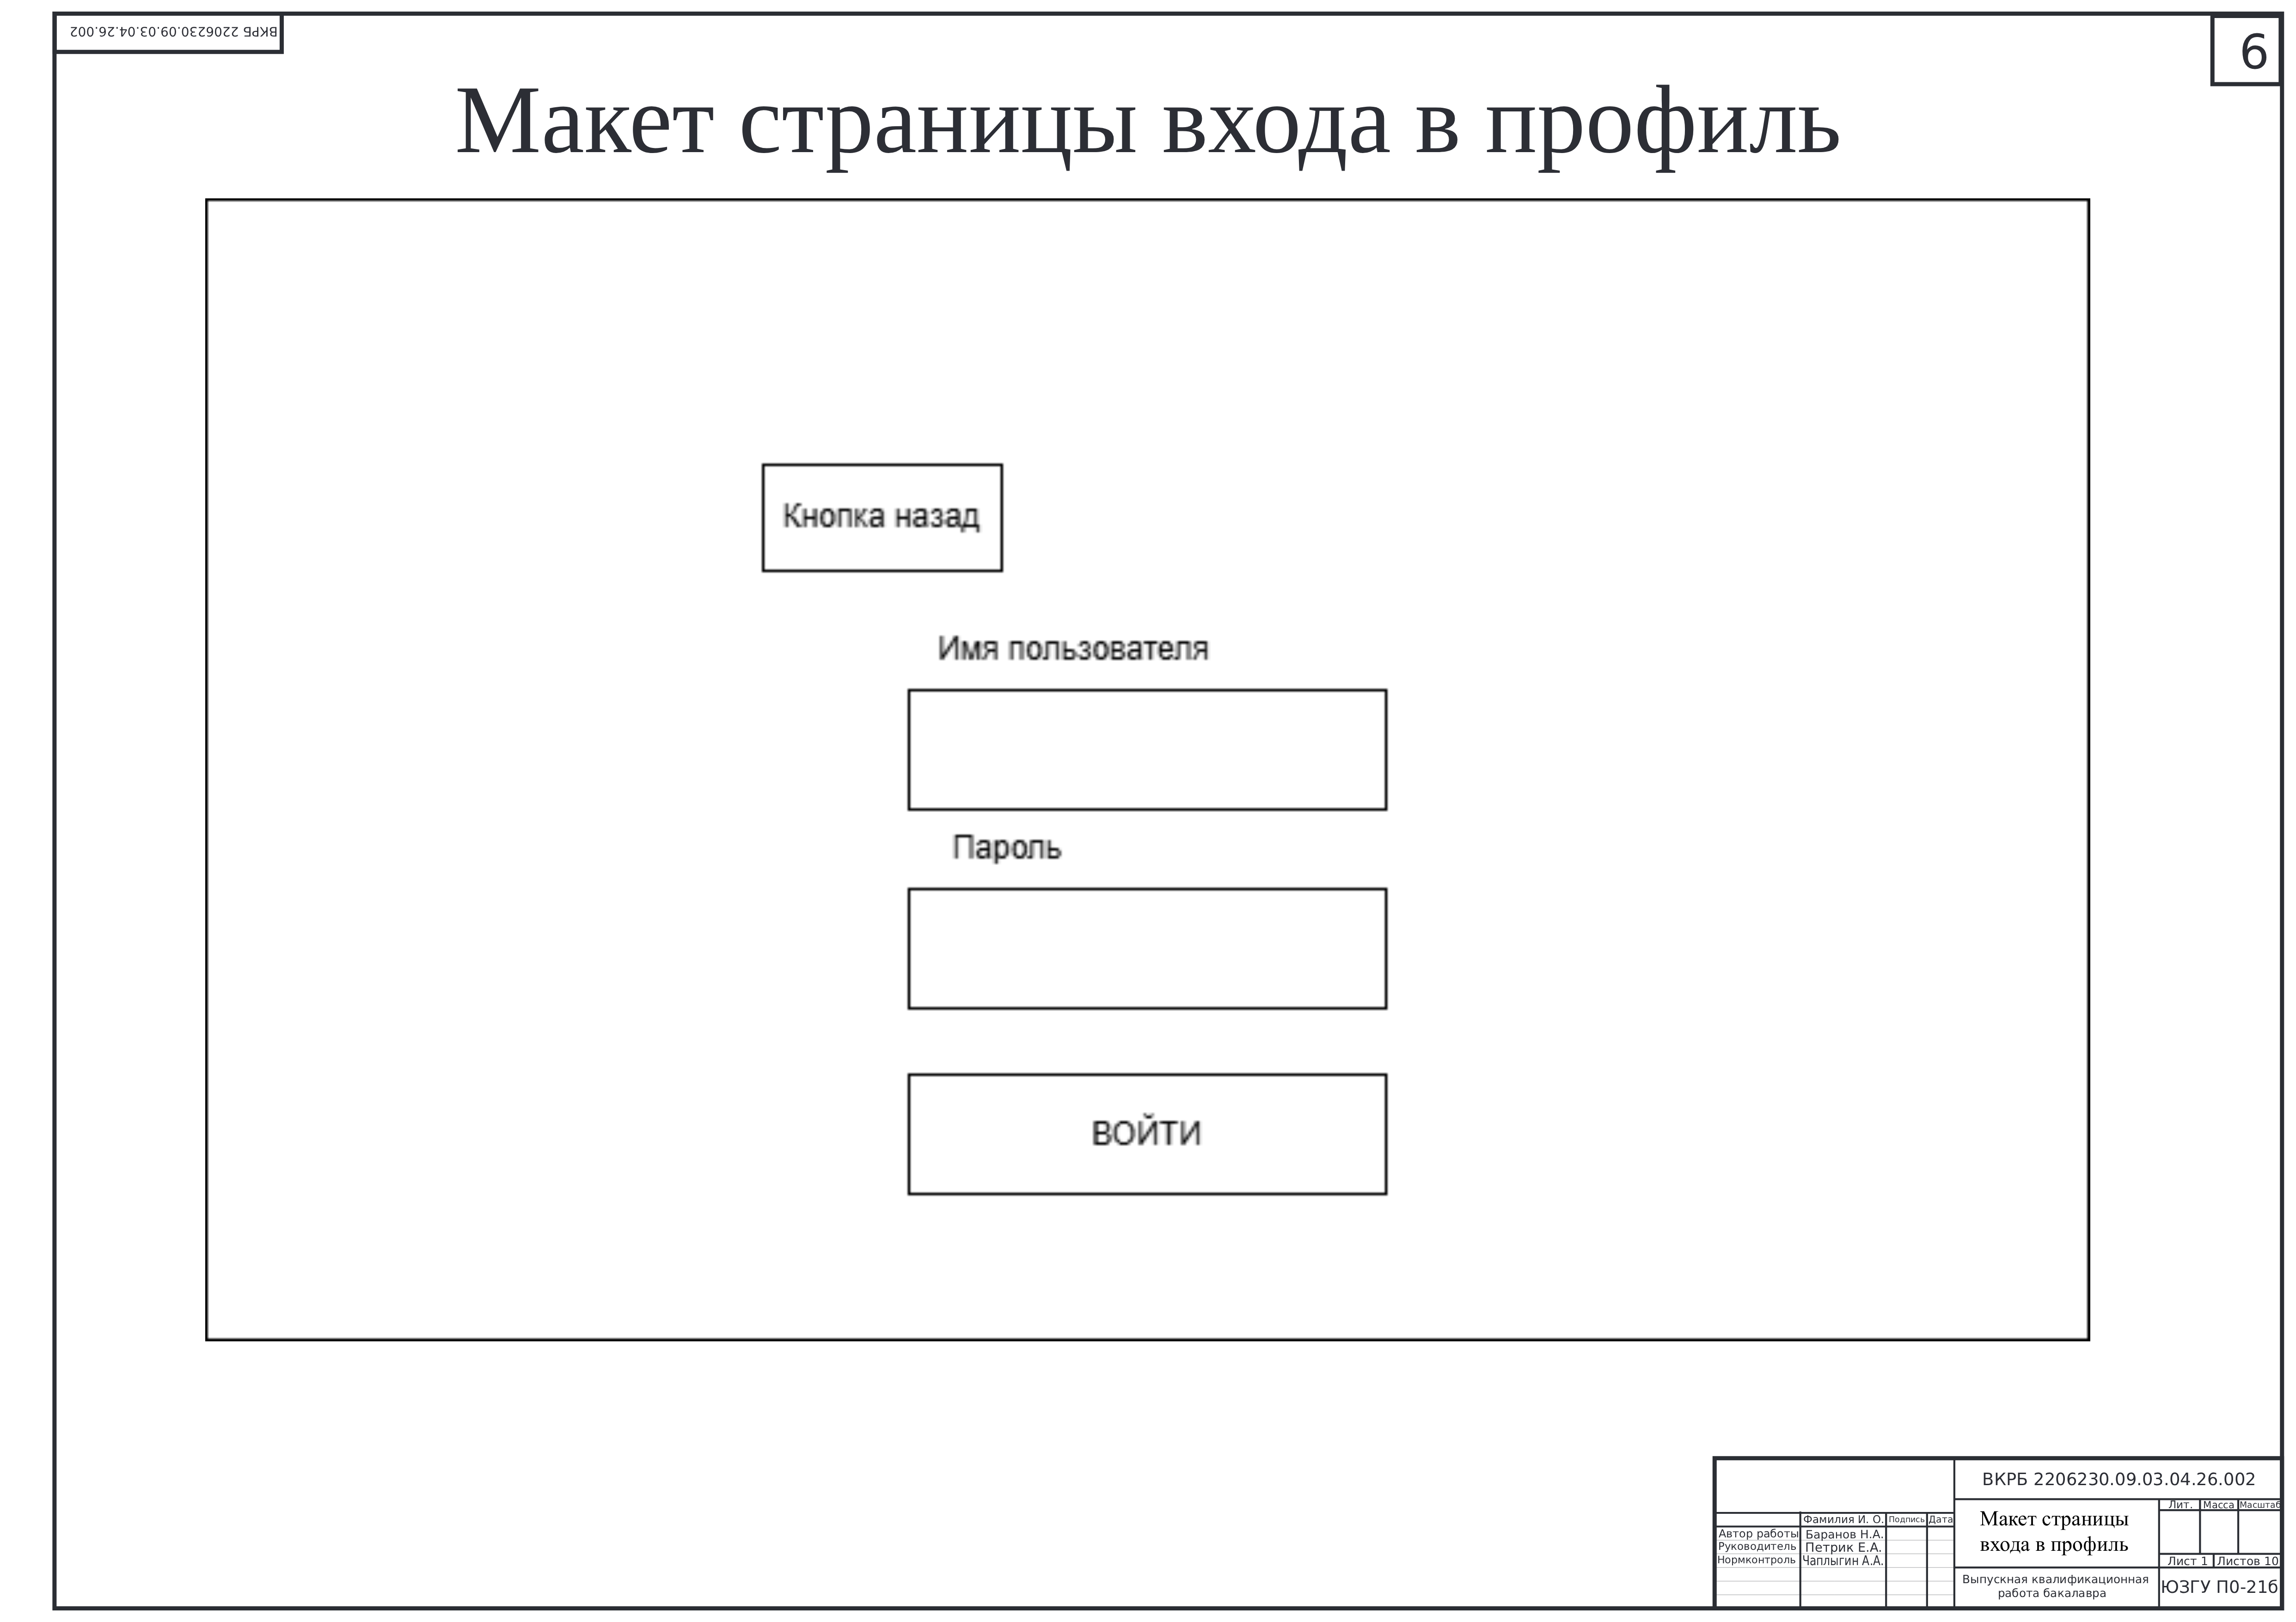
\includegraphics[width=0.82\linewidth]{enter.png}
    \заголовок{Макет страницы входа в профиль}
    \label{pl6:image}      
\end{плакат}

\begin{плакат}
    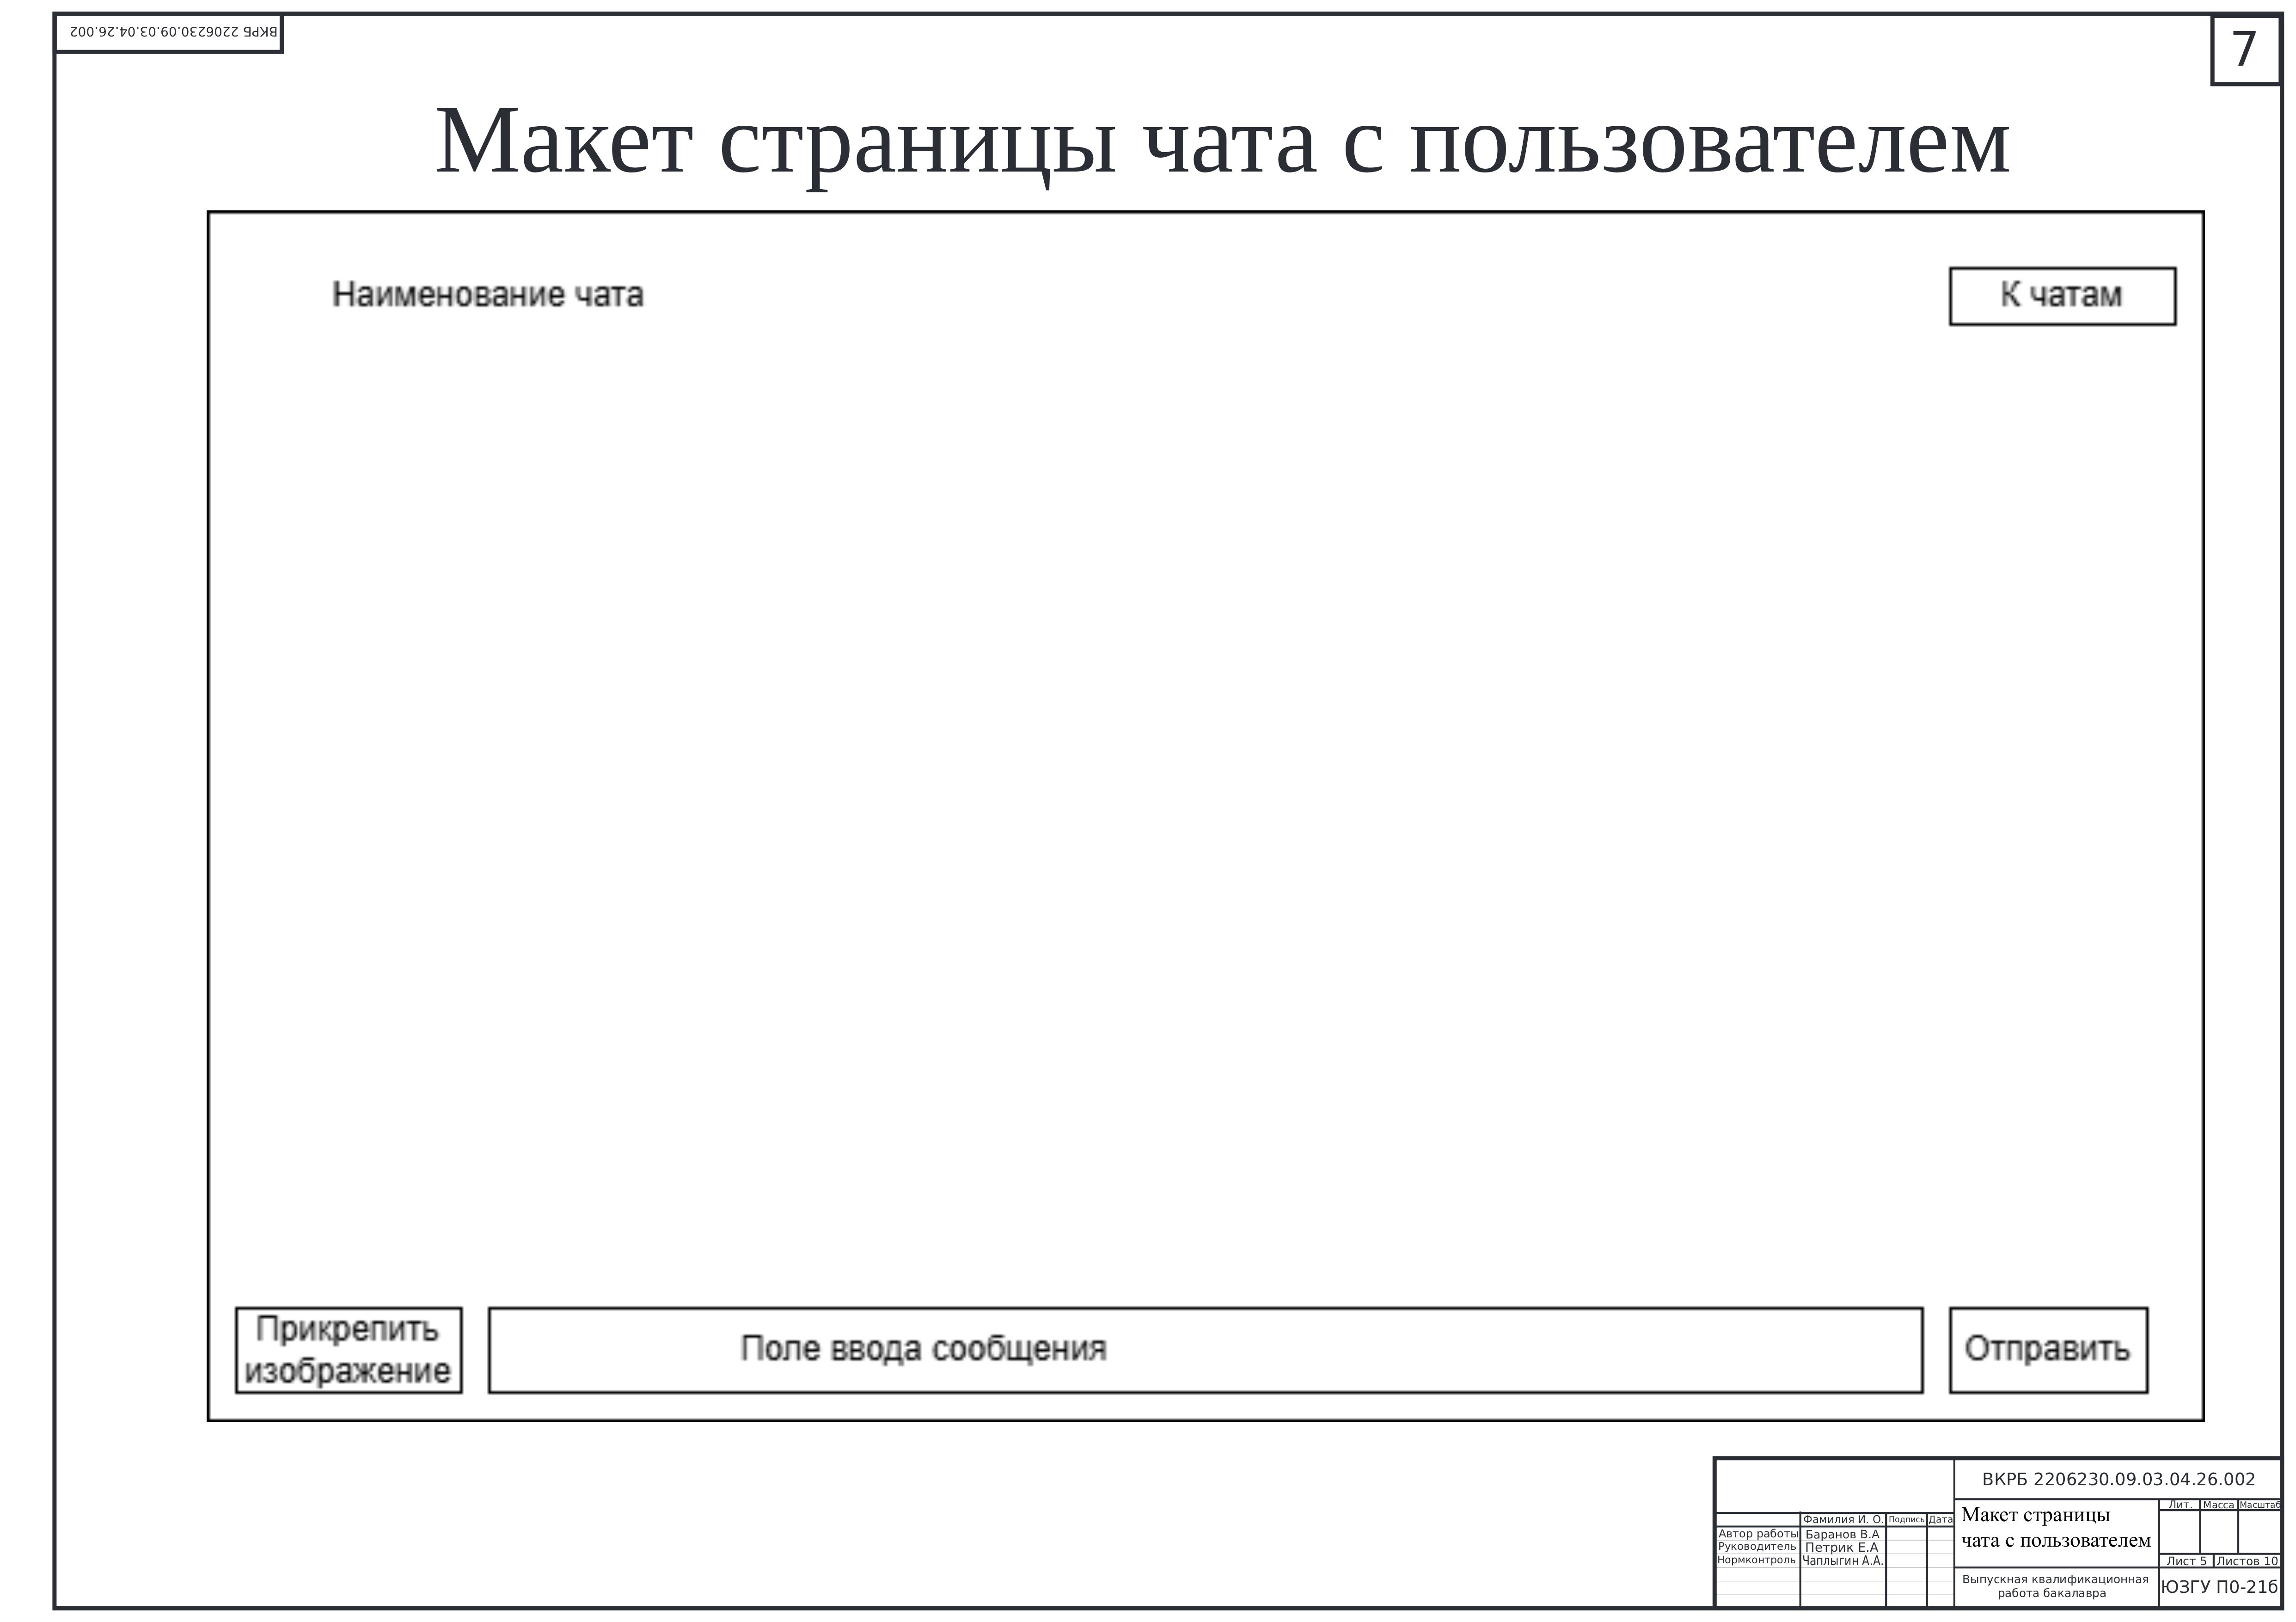
\includegraphics[width=0.82\linewidth]{chats.png}
    \заголовок{Макет страницы чата с пользователем}
    \label{pl7:image}      
\end{плакат}

\begin{плакат}
    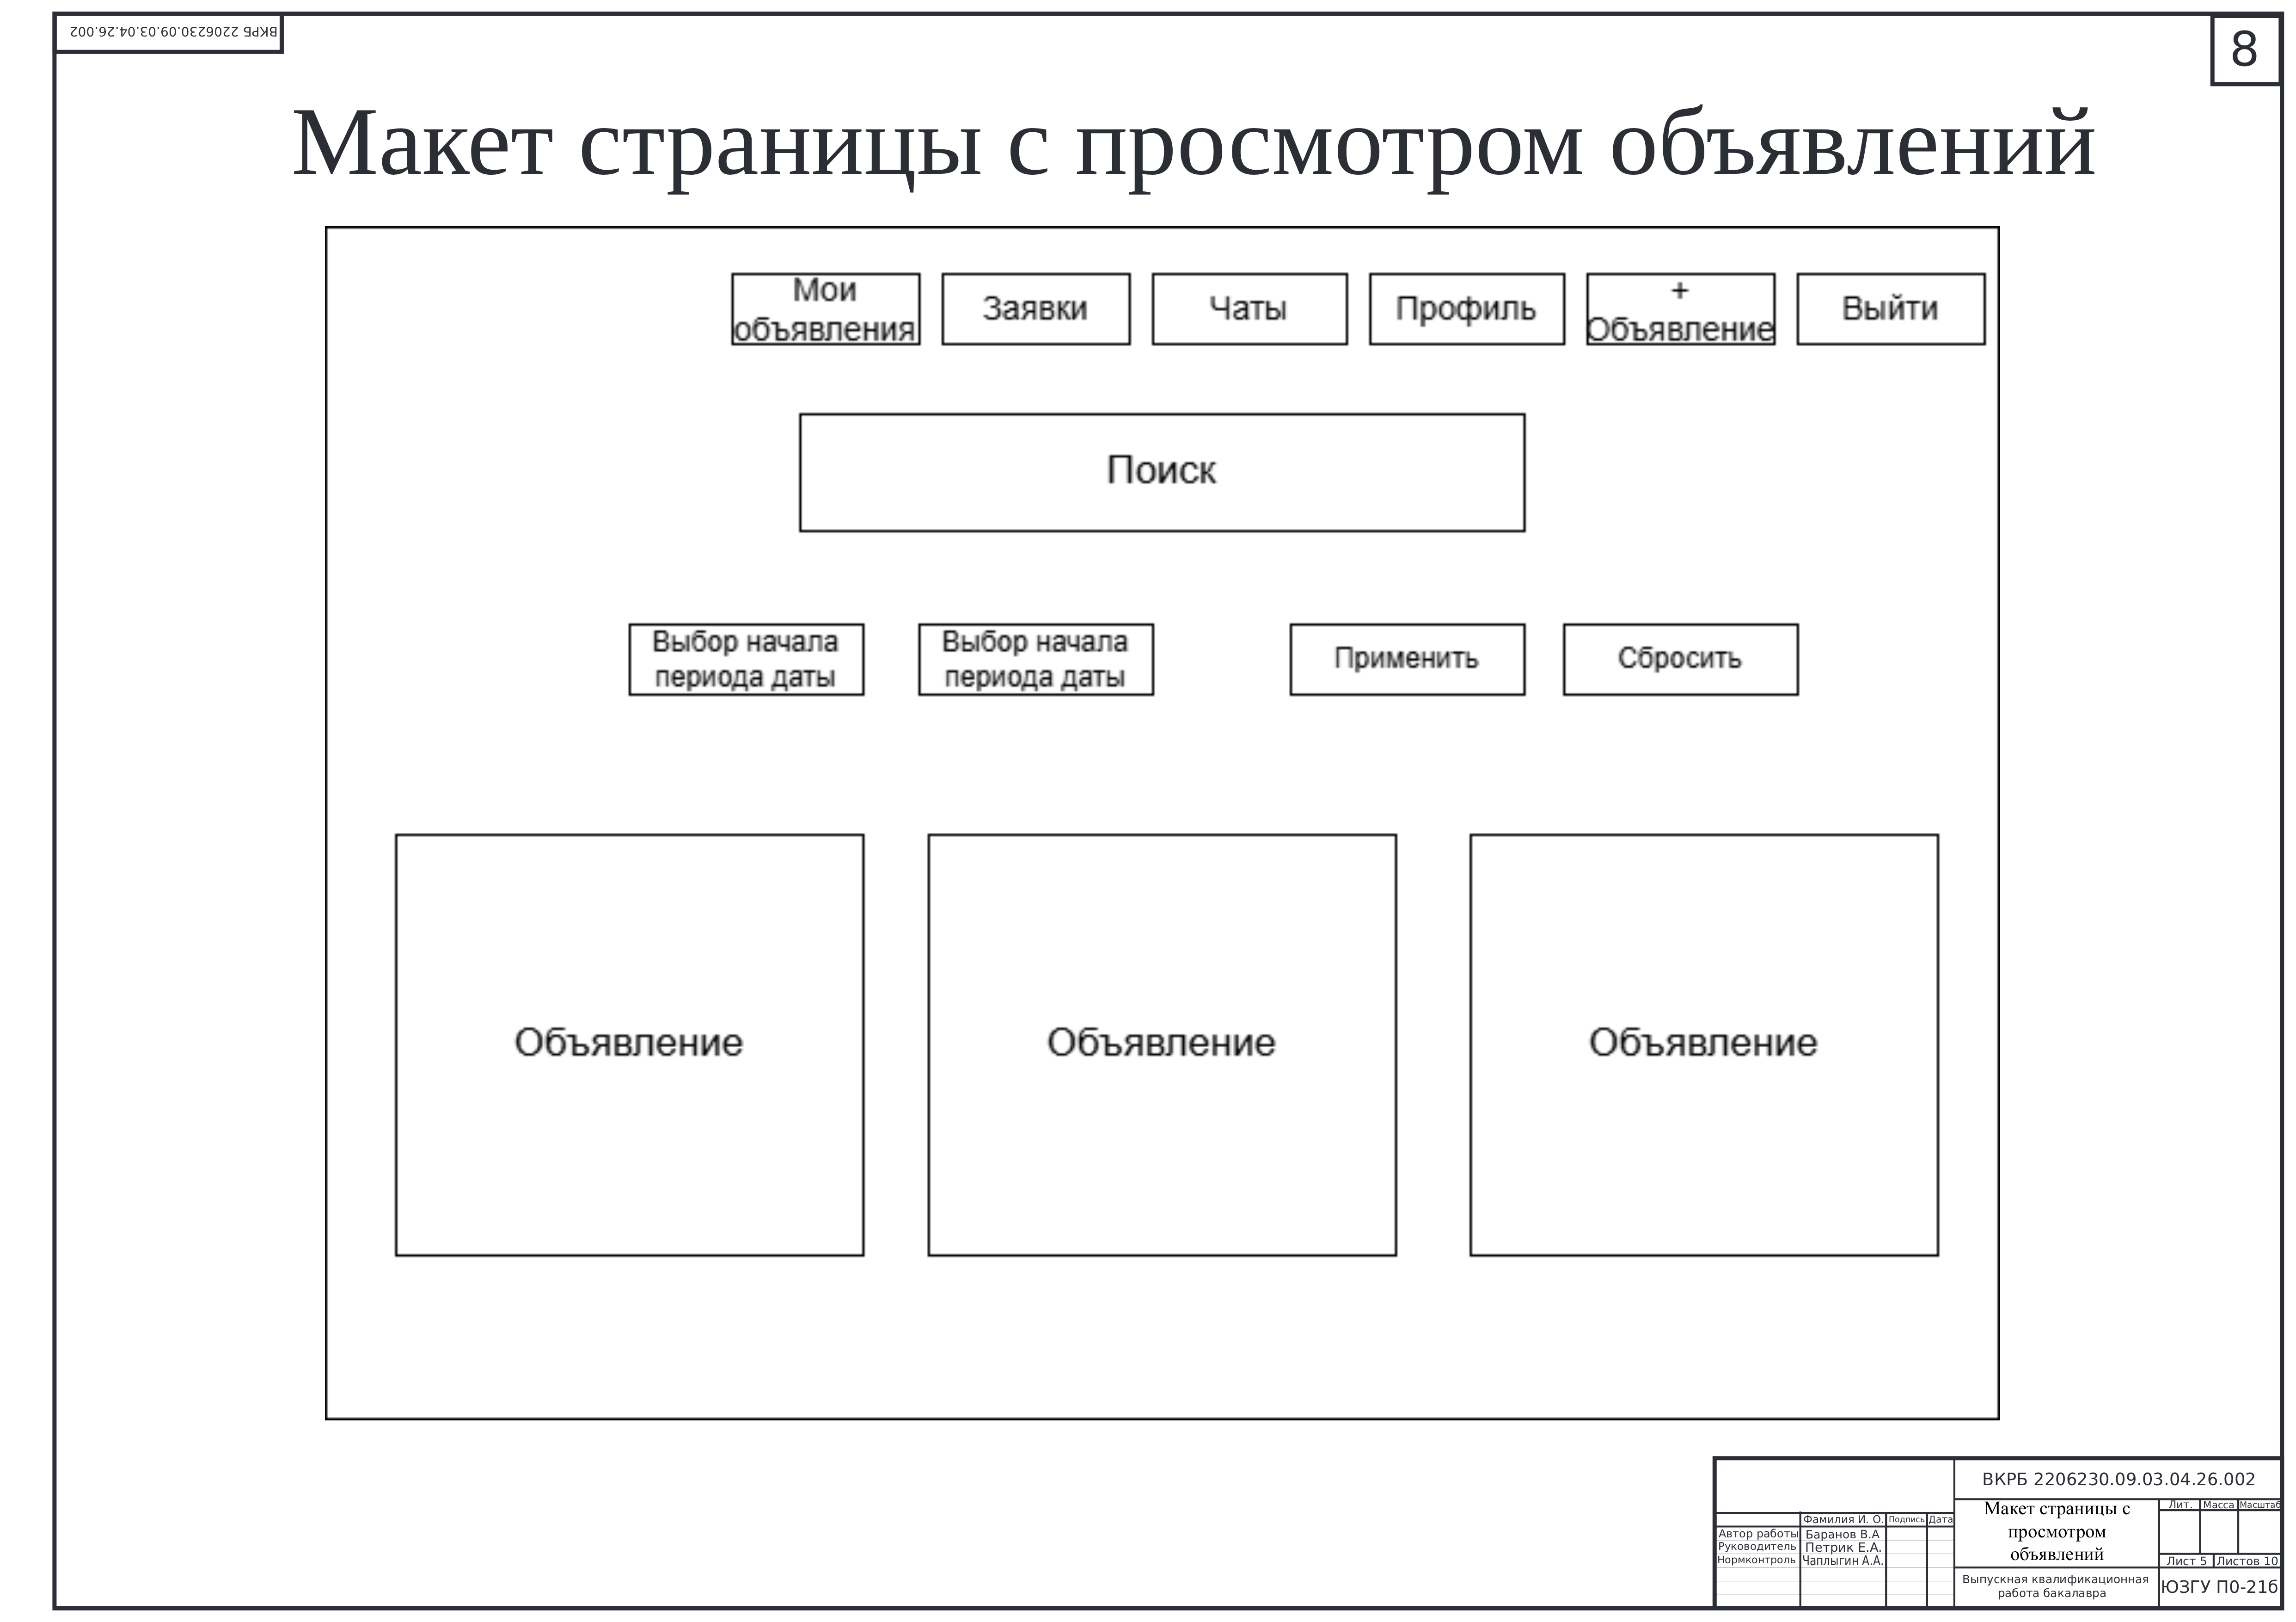
\includegraphics[width=0.82\linewidth]{glavnaya.png}
    \заголовок{Макет страницы просмотра объявлений}
    \label{pl8:image}      
\end{плакат}

\begin{плакат}
    \includegraphics[width=0.82\linewidth]{objavlenie.png}
    \заголовок{Макет страницы информации об объявлении}
    \label{pl9:image}      
\end{плакат}

\begin{плакат}
    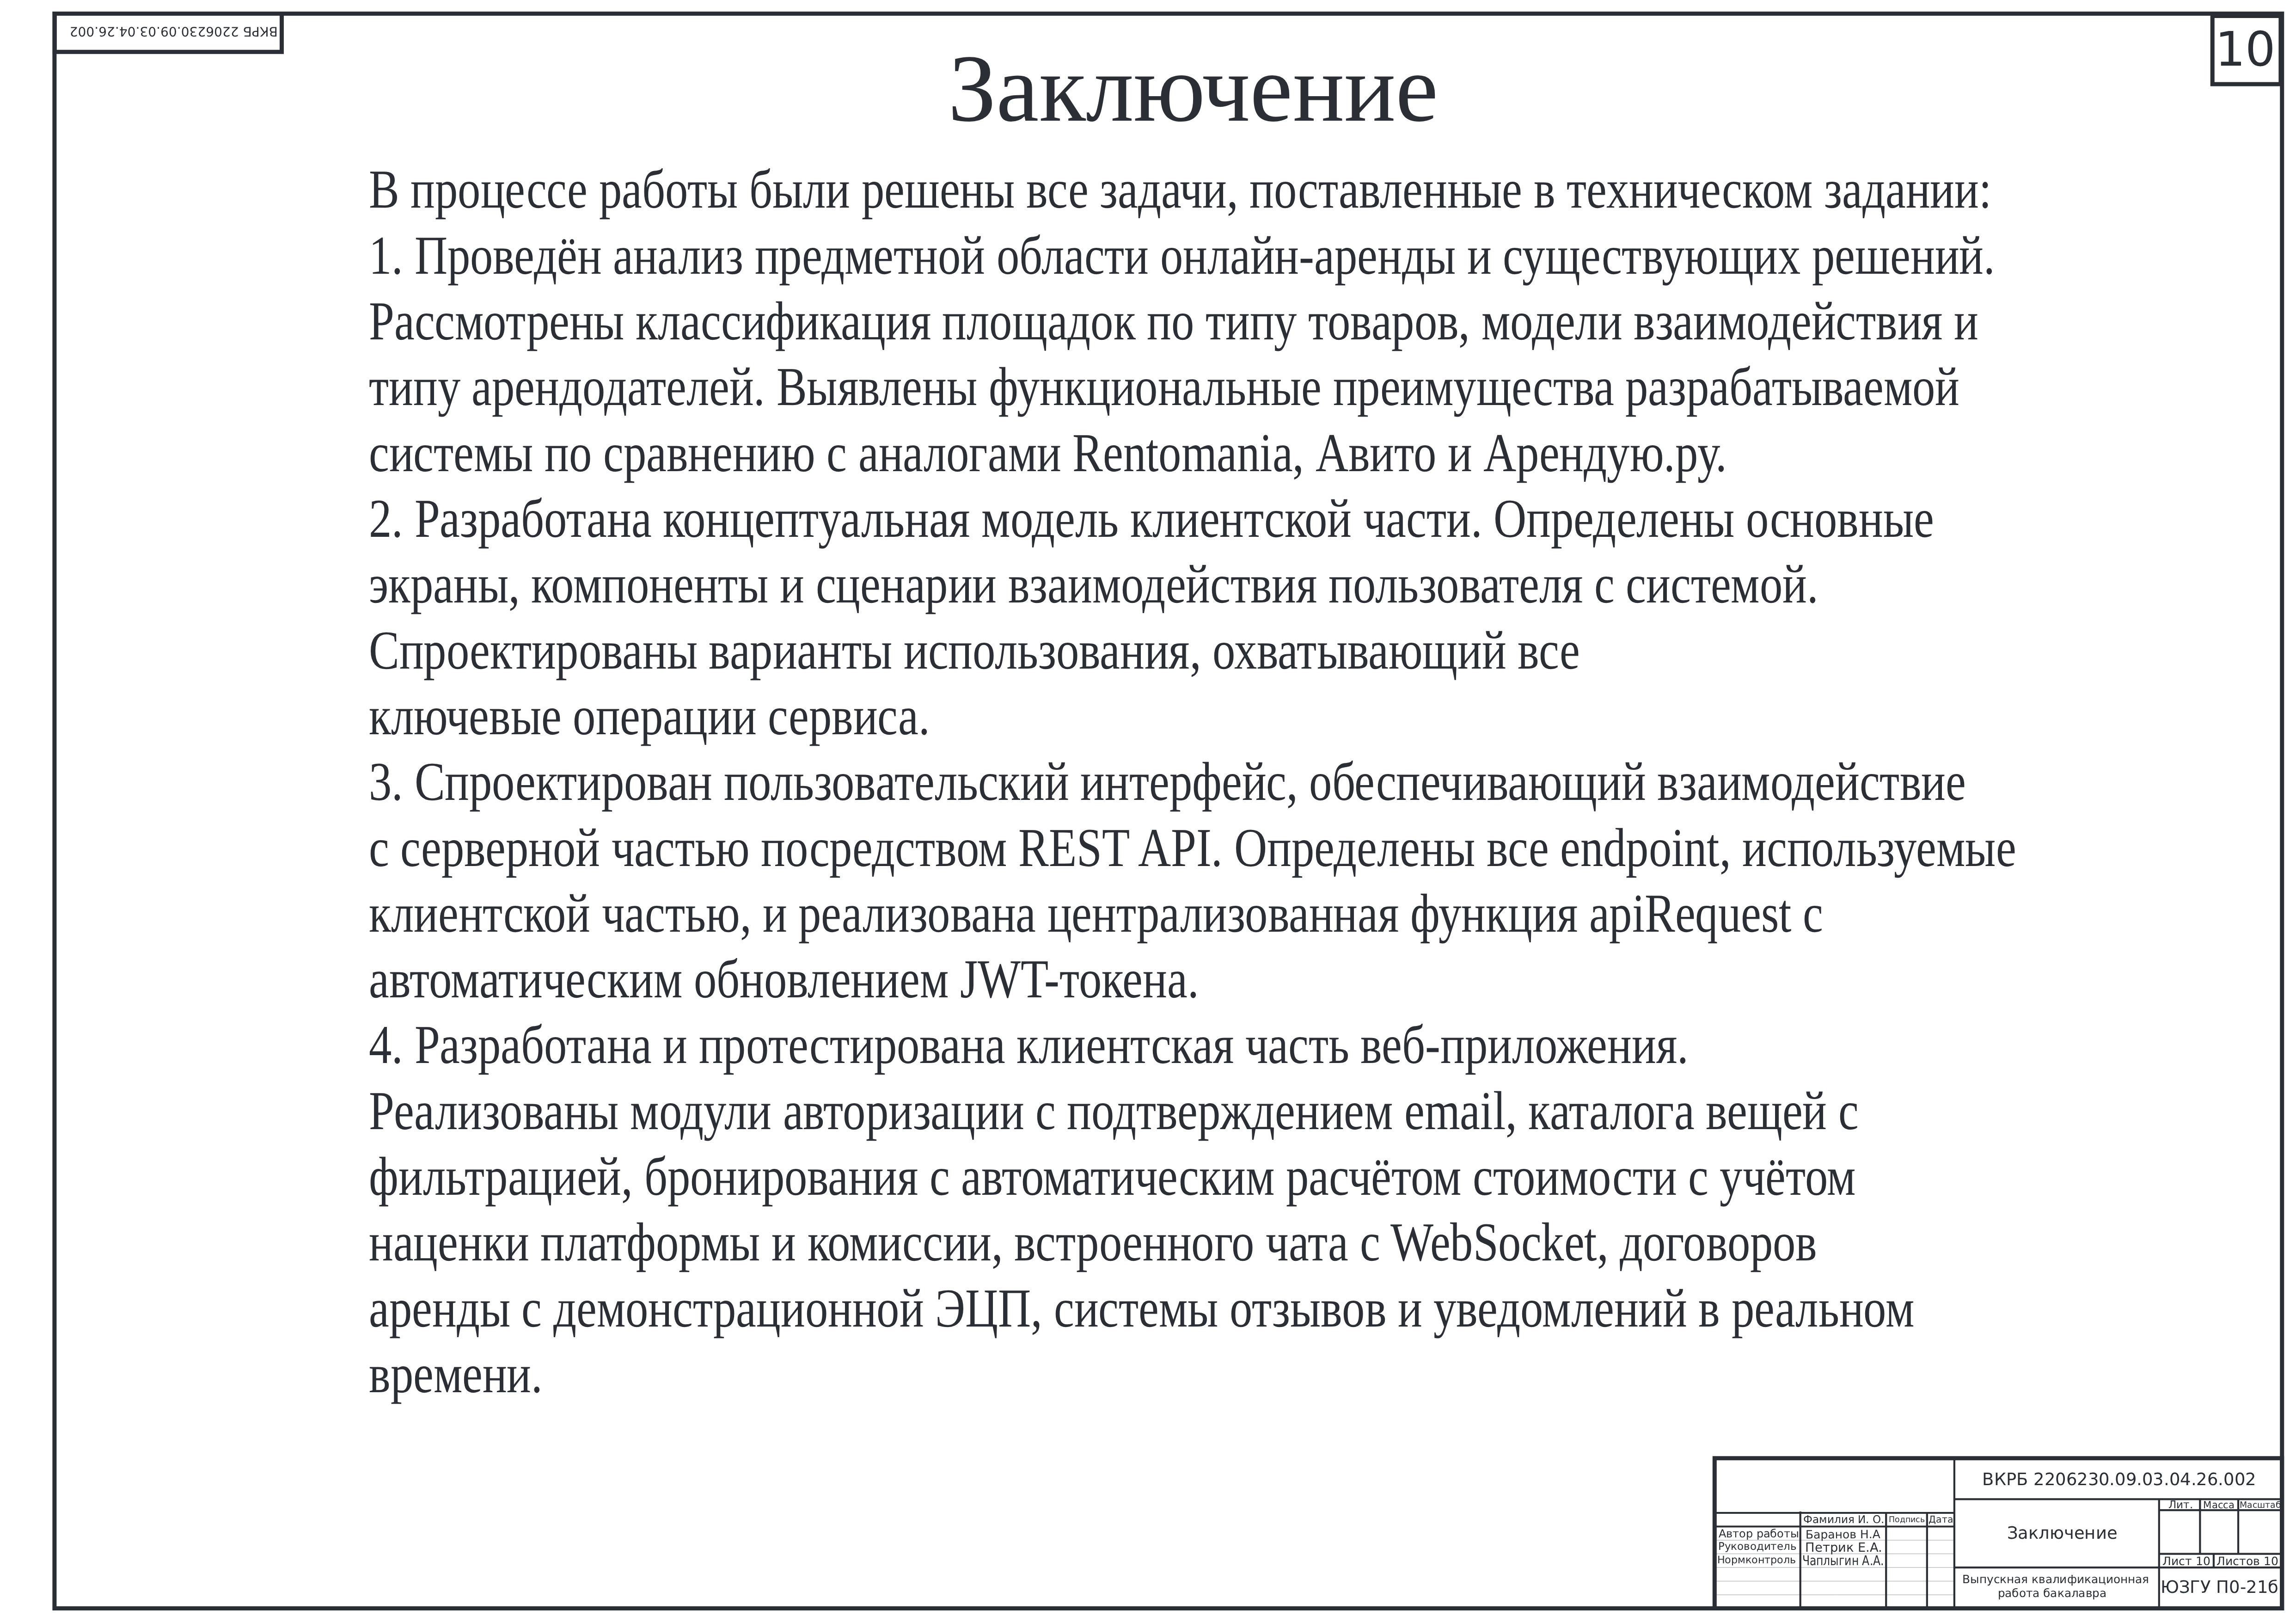
\includegraphics[width=0.82\linewidth]{end.png}
    \заголовок{Заключение}
    \label{pl10:image}      
\end{плакат}

\end{landscape}
